\chapter{Methods} \label{chap:methods}
The methods are introduced in this chapter. Section \ref{sec:classification_method} describes how classification, learning and evaluation procedures are performed. In \cref{sec:network_pruning} the developed network pruning algorithm is introduced and also the dimensionality reduction in pruned networks is shown. Section \ref{sec:insight_of_neural_network} comes with the feature selection method using a procedure called \textit{pathing} and, additionally, some ideas of how to use remaining weights in minimal structures are suggested. Finally, \cref{sec:speech_data_gathering} is devoted to the process of how the speech data was gathered.

Section \ref{sec:classification_method} moreless specifies a generally known approach. Sections \ref{sec:network_pruning} - \ref{sec:insight_of_neural_network} are partially based on \citep{bulin_2016}, but the methods are further elaborated. Section \ref{sec:speech_data_gathering} is highly supported by \citep{smidl_pc}.

\section{Classification Method} \label{sec:classification_method}
The classification in this study is performed by dense feedforward neural networks. An illustration of a general feedforward network structure is in \cref{fig:methods:ff_neural_net}. Note that the structure is fully connected, meaning that each neuron is connected to all neurons in the next layer.

\begin{figure}[H]
\centering
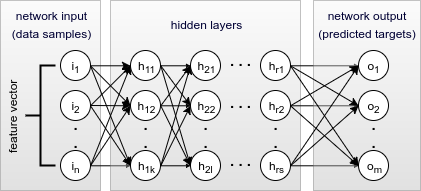
\includegraphics[width=0.9\textwidth]{ff_neural_net}
\caption{A general dense feedforward neural network.}
\label{fig:methods:ff_neural_net}
\end{figure}

The number of input units $ n $ is determined by the problem dimension. The number of classes $ m $ gives the number of output units (see the established conventions in \cref{app:implementation}). In this study, we mostly use a simple hidden structure, usually with one hidden layer ($ q = 1 $).

\subsection*{Neuron Principle}
The behaviour of artificial neurons follows our understanding of how biological neurons work. One unit has multiple inputs and a single output \citep{article:perceptron}. A model of neuron is shown in \cref{fig:methods:model_neuron}. The diagram complies with the following notation:

\begin{description}
\item[$ neuron_k^{(i)} $] : $ k^{th} $ neuron in $ i^{th} $ layer
\item[$ a_k^{(i)} $] : activity of $ k^{th} $ neuron in $ i^{th} $ layer
\item[$ w_{k,l}^{(i)} $] : weight of synapse connecting $ l^{th} $ neuron in $ (i-1)^{th} $ layer with $ k^{th} $ neuron in $ i^{th} $ layer
\item[$ b_k^{(i)} $] : bias connected to $ k^{th} $ neuron in $ i^{th} $ layer
\item[$ z_k^{(i)} $] : activation of $ k^{th} $ neuron in $ i^{th} $ layer
\item[$ f(\cdot) $] : transfer function (\cref{eq:sigmoid}; \cref{fig:methods:transfer_functions})
\end{description}

\begin{figure}[H]
  \centering
  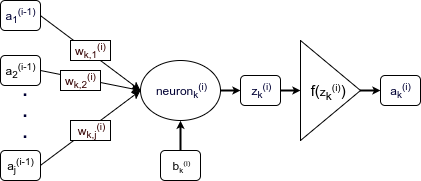
\includegraphics[width=0.9\textwidth]{neuron_principle.png}
  \caption{A model neuron}
  \label{fig:methods:model_neuron}
\end{figure}

Assuming $ j $ being the number of neurons in $ (i-1)^{th} $ layer, the activation of $ neuron_k^{(i)} $ is computed as in \cref{eq:neuron_activation}

\begin{align} \label{eq:neuron_activation}
z_k^{(i)} = \displaystyle{\sum_{l=1}^{j} [a_l^{(i-1)} \cdot w_{k,l}^{(i)}]} + b_k^{(i)}
\end{align}

Then we get the neuron activity by mapping its activation into a finite interval using a transfer function $ f(\cdot) $ - see \cref{eq:neuron_activity}. 

\begin{align} \label{eq:neuron_activity}
a_k^{(i)} = f(z_k^{(i)})
\end{align}

The \textit{Sigmoid} function (\cref{eq:sigmoid}) keeps neuron activities in the $ \langle0, 1\rangle $ interval and is used by default in this work. Alternatively, one could use the hyperbolic tangent ($ tanh(\cdot) $) function, which maps the input into the $ \langle-1, 1\rangle $ interval.

\begin{align} \label{eq:sigmoid}
f(z) = \frac{1}{1 + e^{-z}}
\end{align}

The two basic transfer functions are shown in \cref{fig:methods:transfer_functions}.

\begin{figure}[H]
  \centering
  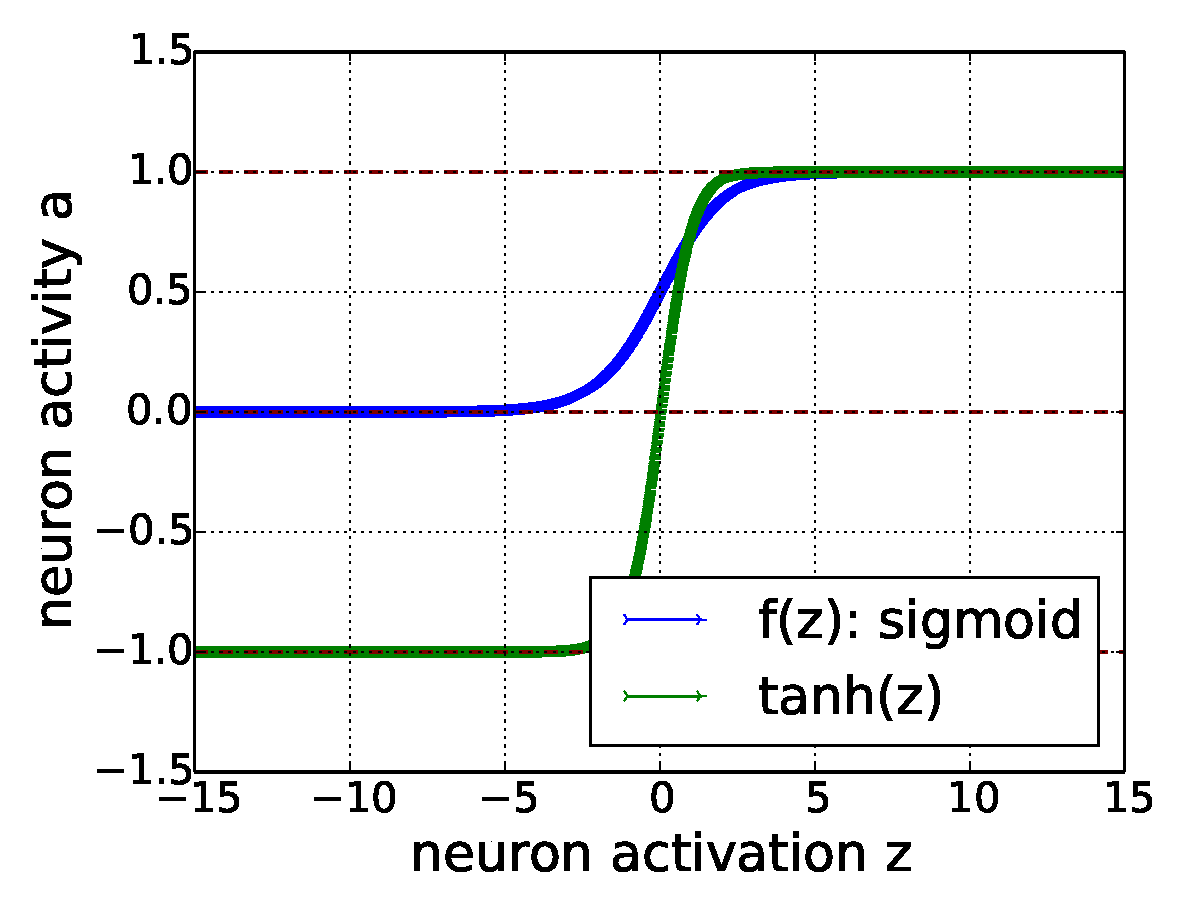
\includegraphics[width=0.7\textwidth]{transfer_functions.eps}
  \caption{Transfer functions: \textit{Sigmoid} and \textit{Tanh}}
  \label{fig:methods:transfer_functions}
\end{figure}

\subsection*{Notation}
The work of a neural network is all done by matrix calculations. Therefore we need to introduce a notation used in this study. Detailed examples of the itemized matrices can be found in \cref{app:implementation}.

\begin{description}[leftmargin=!,labelwidth=\widthof{\bfseries $ W^{(i)} $}]
\item[$ n $] : number of input neurons (problem dimension; size of one sample);
\item[$ m $] : number of output neurons (classes);
\item[$ p $] : number of samples;
\item[$ q $] : number of hidden layers;
\item[$ X $] : network input: $ n $-by-$ p $ matrix;
\item[$ W^{(i)} $] : $ r $-by-$ s $ matrix of weights for synapses connecting $ s $ neurons in $ (i-1)^{th} $ layer to $ r $ neurons in $ i^{th} $ layer;
\item[$ B^{(i)} $] : vector of $ r $ biases for $ r $ neurons in $ i^{th} $ layer;
\item[$ Z^{(i)} $] : $ r $-by-$ p $ matrix of activations for $ r $ neurons in $ i^{th} $ layer for all samples;
\item[$ A^{(i)} $] : $ r $-by-$ p $ matrix of activities of $ r $ neurons in $ i^{th} $ layer for all samples;
\item[$ \Delta^{(i)} $] : $ r $-by-$ p $ matrix of errors on $ r $ neurons in $ i^{th} $ layer for all samples;
\item[$ Y $] : predicted network output for all samples: $ m $-by-$ p $ matrix ($ Y = A^{(q)} $)
\item[$ U $] : desired network output (targets) for all samples: $ m $-by-$ p $ matrix
\end{description}

\subsection*{Learning Algorithm}
Feedforward networks are trained by the common \textit{Backpropagation} method illustrated by the flowchart in \cref{fig:methods:backpropagation}.

\begin{figure}[H]
  \centering
  \includegraphics[width=0.75\textwidth]{backpropagation.png}
  \caption{Training process flowchart. $ T_1 $: Threshold for a terminating condition based on the prediction error (\cref{eq:mse_}). If the error is reduced to be lower $ T_1 $, the learning process is stopped and the model is considered trained. $ T_2 $: Threshold for a terminating condition based on the number of epochs. The learning process is stopped after $ T_2 $ epochs, no matter how successful the training has been.}
  \label{fig:methods:backpropagation}
\end{figure}

In case of feedforward neural networks, the goal is to find optimal values for two groups of parameters - \textit{weights} ($ W $) and \textit{biases} ($ B $). The key idea lies in the optimization method called \textit{Gradient Descent Algorithm (GDA)}.

At first, a batch of samples $ X $ is (forward) propagated through a network to get the network's prediciton $ Y $.

\begin{align}
Z^{(1)} &= W^{(1)} \cdot X + B^{(1)} \\
A^{(1)} &= f(Z^{(1)}) \\
A^{(i)} &= f(W^{(i)} \cdot A^{(i-1)} + B^{(i)}) \\
Y &= A^{(q)} = f(W^{(q)} \cdot A^{(q-1)} + B^{(q)})
\end{align}

Then, having the known targets (supervised learning), we compute a prediction error on every output neuron for every sample and store those errors in the $ m $-by-$ p $ matrix $ E $.

\begin{equation} \label{eq:prediction_error}
E = \frac{1}{2} ||U - Y||^2
\end{equation}

Now it is time to use \textit{GDA} to find such settings of $ W $ and $ B $ that makes $ E $ minimal. The details of the \textit{Backpropagation} procedure are well described in \citep{online:nnanddl}. The envelope of the algorithm includes these steps:

\begin{enumerate}
\item \textit{find the derivative of the transfer function (assuming Sigmoid)};
\begin{align} \label{eq:transfer_function_der}
f'(z) = f(z) \cdot (1-f(z))
\end{align}
\item \textit{backpropagate the prediction error throught the network;}
\begin{align} \label{eq:error_backprop}
\Delta^{(q+1)} &= (U-Y) \times f'[Z^{(q+1)}] \\
\Delta^{(i)} &= \left[\left[W^{(i+1)}\right]^T \cdot \Delta^{(i+1)}\right] \times f'[Z^{(i)}]
\end{align}
\item \textit{find the optimal parameter changes;}

Every sample $ \xi $ has a vote $ dW^{(i)}_{(\xi)} $ (resp. $ dB^{(i)}_{(\xi)} $) on how the parameters $ W^{(i)} $ (resp. $ B^{(i)} $) should change to get the minimal error and the result is then obtained as a compromise of those votes.

Index $ (i) $ indicates the layer. Consider $ \Delta^{(i)}_{(\xi)} $ be the $ \xi^{th} $ column of the $ \Delta^{(i)} $ matrix, which corresponds to the $ \xi^{th} $ sample. Analogically, $ A^{(i-1)}_{(\xi)} $ is the $ \xi^{th} $ column of the activation matrix $ A^{(i-1)} $ in the $ (i-1)^{th} $ layer. Then we get the votes as:
\begin{align} \label{eq:part_derivative}
dW^{(i)}_{(\xi)} &= A^{(i-1)}_{(\xi)} \cdot \left[\Delta^{(i)}_{(\xi)}\right]^T\\
dB^{(i)}_{(\xi)} &= \Delta^{(i)}_{(\xi)}
\end{align}
\item \textit{update the parameters.}

At this point we introduce the first parameter of the learning process called \texttt{batch\_size}. It states how many votes are processed together to make one update of the parameters. If \texttt{batch\_size = 1}, we are talking about a \textit{sequential learning}. In this case, each vote is applied to update the parameters before any other votes are computed (\cref{eq:sequential_update}; $ t $ refers to a moment in time). 

\begin{align} \label{eq:sequential_update}
dW^{(i)}(t) = dW^{(i)}_{(\xi)}
\end{align}

In this work, we usually use \textit{batch learning} ( \texttt{batch\_size > 1}).

\begin{align} \label{eq:batch_update}
dW^{(i)}(t) = \displaystyle{\sum_{\xi}^{batch\_size} dW^{(i)}_{(\xi)}}
\end{align}

Equations \ref{eq:sequential_update} and \ref{eq:batch_update} works analogically for the biases.

The second parameter of the learning procedure is called \texttt{learning\_rate} ($ \mu $) and is usually set $ 0 < \mu << 1 $ in order to deal with GDA problems (see \citep{online:nnanddl}). The update of the parameters is then done as follows:
\begin{align} \label{eq:params_update}
W^{(i)} (t+1) &= W^{(i)} (t) + \mu \cdot dW^{(i)} (t) \\ 
B^{(i)} (t+1) &= B^{(i)} (t) + \mu \cdot dB^{(i)} (t)
\end{align}
\end{enumerate}

When the votes of all samples are applied, the learning epoch ends (see \cref{fig:methods:backpropagation}). The maximal number of epochs and the maximal required error (see \cref{fig:methods:backpropagation}) are also parameters of the learning procedure. To list them all:

\begin{itemize}
\item \texttt{batch\_size}
\item \texttt{learning\_rate} ($ \mu $)
\item \texttt{n\_epoch}
\item \texttt{max\_error} ($ MSE' $; \cref{eq:mse_})
\end{itemize}

\subsection*{Network Evaluation}
We use two measures to evaluate the network training: error and accuracy.
The error measure is based on the standard \textit{Mean Squared Error (MSE)} given by \cref{eq:mse}.

\begin{equation} \label{eq:mse}
MSE = \frac{1}{2 p} \displaystyle{\sum^{p}_{\xi=1} ||y_{\xi} - u_{\xi}||^2}
\end{equation}

where $ y_{\xi} $ is the prediction for sample $ \xi $ and $ u_{\xi} $ its corresponding (known) target. Both are vectors of length $ m $ (number of classes).

In this study we rather use the measure given by \cref{eq:mse_}, because it makes a fair comparison of problems with different number of classes.

\begin{equation} \label{eq:mse_}
MSE' = \frac{1}{2 p m} \displaystyle \sum^{p}_{\xi=1} \displaystyle \sum^{m}_{\theta=1} (y_{\xi,\theta} - u_{\xi,\theta})^2
\end{equation}

The classification accuracy is computed with \cref{eq:acc}.

\begin{equation} \label{eq:acc}
acc = \frac{1}{p} \displaystyle \sum^{p}_{\xi=1} \psi, \qquad \psi = \begin{cases}
    1, & argmax(y_{\xi}) = argmax(u_{\xi}) \\
    0, & \text{otherwise}
\end{cases} 
\end{equation}

The classification result is often shown by a confusion matrix (well explained in \citep{sklearn}. The testing is usually done on different data samples than used for training - see \cref{fig:methods:three_sets}.

\section{Network Pruning} \label{sec:network_pruning}
The rule of thumb in classification with feedforward neural networks is using a fully connected structure - every unit is connected to all units in the next layer. 

Pruning methods work with the hypothesis that some of the synapses in fully connected networks do not contribute to the classification and so their removal would not cause a significant accuracy drop. The problem (graphically illustrated in \cref{fig:methods:pruning_problem_formulation}) is to distinguish those redundant synapses from the important ones.

\begin{figure}[H]
  \centering
  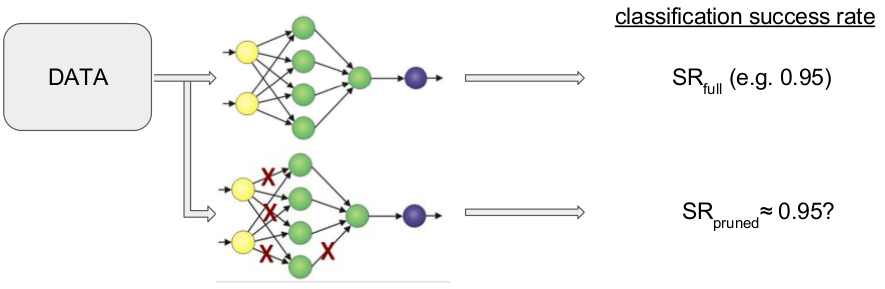
\includegraphics[width=0.9\textwidth]{pruning_problem_formulation}
  \caption{Pruning Algorithm: problem formulation.}
  \label{fig:methods:pruning_problem_formulation}
\end{figure}

There are several ways of how to estimate the importance of synapses (see \cref{sec:state_of_the_art}). In this study we introduce a measure called \textit{weight significance factor} (\texttt{WSF}) given by \cref{eq:weight_significance_factor}.

\begin{equation} \label{eq:weight_significance_factor}
WSF(w_{k,l}^{(i)}) = | w_{k,l}^{(i)} (t_f) - w_{k,l}^{(i)} (0) |
\end{equation}

where $ w_{k,l}^{(i)} (t_f) $ is the weight of synapse coming to $ k^{th} $ neuron in the $ i^{th} $ layer from $ l^{th} $ neuron in $ (i-1)^{th} $ layer after training ($ t_f $: time final). Analogically, $ w_{k,l}^{(i)} (0) $ is the initial weight of the same synapse before training. We compare these two values and get the change in weight over the training process. The key idea is that the redundant synapses do not change their weights over the training. Therefore, those synapses with low \texttt{WSF} are considered less important than those with high \texttt{WSF}.

\subsection*{Realization of the Pruning Proceeder}
The general recipe of how to prune a synapse is illustrated in \cref{fig:methods:network_pruning_flowchart}.

\begin{figure}[H]
  \centering
  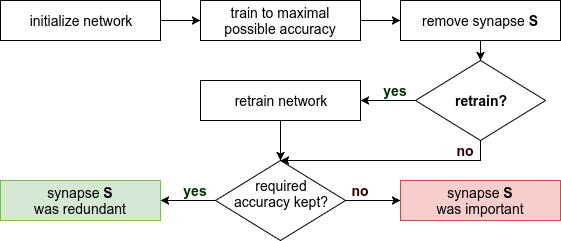
\includegraphics[width=0.75\textwidth]{network_pruning_flowchart}
  \caption{The flowchart of pruning one synapse, demonstration of parameter \texttt{retrain}.}
  \label{fig:methods:network_pruning_flowchart}
\end{figure}

\cref{fig:methods:network_pruning_flowchart} introduced the first parameter of the pruning process called \texttt{retrain}. We make it $ True $ if we want to retrain the pruned network (without the cut synapse) before checking the accuracy drop. In practice, we are able to set the exact number of epochs we want the net to retrain.

The required accuracy (\texttt{req\_acc}) is the second parameter. In some cases we want to give up some of the accuracy in exchange for well pruned network in order to see some patterns in it. This parameter sets the minimal accuracy the network must have so that we can treat the lastly cut synapses as unimportant. The accuracy is checked on development data, while the training is performed on training data (see \cref{fig:methods:three_sets}).

So far we gave a recipe of how to prune one synapse. Of course, we cannot check all the synapses one by one using the approach in \cref{fig:methods:network_pruning_flowchart}. Instead we cut out multiple synapses at once before checking the accuracy drop. In fact, network pruning is an iterative procedure with some guessing. The first guess is the order in which we prune the synapses and the second guess is how many should we prune at once.

The order of the synapses is dermined by the \texttt{WSF} (\cref{eq:weight_significance_factor}) - the key idea of our pruning algorithm. Each time before pruning, all the synapses are sorted by their \texttt{WSF} values.

To estimate the number of synapses to cut at once we use percentiles - see \cref{fig:methods:network_pruning_proceeder}.

\begin{figure}[H]
  \centering
  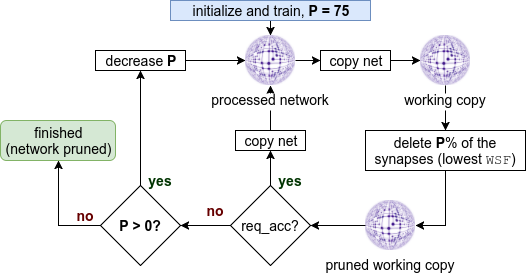
\includegraphics[width=0.75\textwidth]{network_pruning_algorithm}
  \caption{Network pruning proceeder.}
  \label{fig:methods:network_pruning_proceeder}
\end{figure}

The percentile level is set to $ P = 75 $ at the beginning. Hence the algorithm tries to prune $ 75\% $ of the synapses (those with low \texttt{WSF}) in the first pruning step. Then the accuracy drop is checked (with or without retraining). If the accuracy dropped, we decrease the percentile level $ P $ and try to delete less synapses in the next step.

At this point we introduce another parameter of the pruning procedure called \texttt{percentile\_levels}, which is an array specifying the levels we try (e.g.  $percentile\_levels = (75, 50, 30, 20, 0) $). The last level in this array is always zero. When $ P = 0 $ we delete only the one synapse; the one with the lowest \texttt{WSF}. In this manner, at some point of the pruning process, the algorithm will come to removing only one synapse at once and if only a single synapse has been removed during the last pruning step and the accuracy has been broken, it means that even this single synapse with the least change in weight is important for classification. Therefore, the pruning is stopped and the current net structure (including this last synapse) is saved as the minimal structure. Therefore, the algorithm is finite and it also guarantees that the classification accuracy does not drop. To sum up the parameters of the pruning procedure:

\begin{itemize}
\item \texttt{retrain}
\item \texttt{req\_acc}
\item \texttt{percentile\_levels}
\end{itemize}

\subsection*{Dimensionality Reduction}
In practise, neural networks are usually represented by matrices ($ W $ and $ B $) and the learning and prediction are performed by matrix calculations. The pruning algorithm cuts out some synapses which leads to the reduction of matrix dimensions if we restructure the matrices after pruning.

If a synapse is pruned, the corresponding weight in the $ W $ matrix takes zero value. Consider the following weight matrix $ W^{(i)} $, where the $ i^{th} $ layer consists of $ 3 $ neurons and the $ (i-1)^{th} $ layer has $ 4 $ neurons.
\begin{align*}
W_{full}^{(i)} = 
\begin{bmatrix}
    w_{11}^{(i)} & w_{12}^{(i)} & w_{13}^{(i)} & w_{14}^{(i)} \\
    w_{21}^{(i)} & w_{22}^{(i)} & w_{23}^{(i)} & w_{24}^{(i)} \\
    w_{31}^{(i)} & w_{32}^{(i)} & w_{33}^{(i)} & w_{34}^{(i)}
\end{bmatrix}
=
\begin{bmatrix}
    -0.02 & 0.32 & -0.28 & -0.91 \\
    -0.72 & 0.9 & 0.81 & 0.54 \\
    0.13 & -0.45 & 0.62 & 0.24
\end{bmatrix}
\end{align*}
Now, let's assume that synapses corresponding to weights $ w_{13}^{(i)} $, $ w_{14}^{(i)} $, $ w_{21}^{(i)} $, $ w_{22}^{(i)} $, $ w_{23}^{(i)} $, $ w_{24}^{(i)} $, $ w_{31}^{(i)} $, $ w_{33}^{(i)} $ were pruned. The weight matrix $ W^{(i)} $ changes to:
\begin{align*}
W_{pruned}^{(i)} = 
\begin{bmatrix}
    -0.02 & 0.32 & 0 & 0 \\
    0 & 0 & 0 & 0 \\
    0 & -0.45 & 0 & 0.24
\end{bmatrix}
\end{align*}
We know that each row of the matrix corresponds to inputs of one neuron in the $ i^{th} $ layer and each column maps the outputs of one neuron in the $ (i-1)^{th} $ layer. Therefore, if we find a row of zeros, we can safely remove the corresponding ($ 2^{nd} $) neuron from the network, as it has no inputs. Moreover, we can (better said we must) also remove the $ 2^{nd} $ column in the weight matrix $ W^{(i+1)} $ responsible for the outputs of the removed neuron.

Analogically, if the $ 3^{rd} $ neuron in the $ (i-1)^{th} $ layer has no outputs ($ 3^{rd} $ column of zeros in $ W^{(i)} $), it is useless for classification. Hence we can also delete this column in $ W^{(i)} $ and must remove corresponding inputs of the removed neuron, which is the $ 3^{rd} $ row of the weight matrix $ W^{(i-1)} $. We call the process network shrinking.
\begin{align*}
W_{shrinked}^{(i)} = 
\begin{bmatrix}
    -0.02 & 0.32 & 0 \\
    0 & -0.45 & 0.24
\end{bmatrix}
\end{align*}
After the removal of a specified neuron, a corresponding bias is also removed. When we shrink the first hidden layer, we must also adjust the feature vectors accordingly.

\section{Insight of Neural Network} \label{sec:insight_of_neural_network}
We know that state-of-the-art fully-connected networks can be trained to work very well for several tasks, however hardly ever we know why they work so well. Pruned networks come with some advantages that help demystify these black-box models.

\subsection*{Pathing in Networks}
Based on the PA (\cref{sec:network_pruning}) we assume that every single synapse left in the pruned network is somehow important for classification. Therefore it makes sense to track these connections from the input to the output of a network to find out some patterns among features and classes. We define $ path_f^{(c)} $ as a sorted list of synapses that connects feature $ f $ with class $ c $ (\cref{fig:methods:path_explanation}).

\begin{figure}[H]
  \centering
  \includegraphics[width=0.45\textwidth]{path_explanation}
  \caption{Explanation of a path.}
  \label{fig:methods:path_explanation}
\end{figure}

If there is a path from feature $ f_1 $ to class $ c_1 $, we assume that $ f_1 $ is interesting for the class. Otherwise, if there is no path, the feature is probably not needed for class $ c_1 $ at all. This leads to a promising idea of how to do feature selection.

\subsection*{Feature Energy}
Moreover, we also know the weights of the remaining synapses. Hence, besides the information if or if not a feature influences some class, we can also state how big the influence is. We introduce a measure called \textit{feature energy} (\texttt{E}).

\begin{equation} \label{eq:feature_energy}
E(f,c) = \displaystyle{\sum_{p=1}^{P} \displaystyle{\prod_{s=1}^{S_p} \frac{w_s^{(p)}}{|b_s^{(p)}|}}}
\end{equation}

where $ E(f,c) $ is the energy of feature $ f $ for class $ c $, $ P $ is the number of paths from feature $ f $ to class $ c $, $ S_p $ is the number of synapses in the $ p^{th} $ path, $ w_s^{(p)} $ is the weight of the $ s^{th} $ synapse in the $ p^{th} $ path and $ b_s^{(p)} $ is the bias of the neuron this synapse is connected to.

A total energy $ E(f) $ of feature $ f $ for a classification problem is given as:

\begin{equation} \label{eq:feature_energy_total}
E(f) = \displaystyle{\sum_{k=1}^{m} | E(f,c_k)} |
\end{equation}

\newpage
\section{Speech Data Gathering} \label{sec:speech_data_gathering}
The presented methods are tested on several examples (\cref{chap:examples}) and one of them rests in classification of phonemes. By definition a phoneme is one of the units of sound that distinguish one word from another in a particular language \citep{wiki:mnist}. We focus on Czech language and consider $ 40 $ phonemes listed in \cref{tab:methods:phonetic_alphabet}. This section describes the way of gathering such phonemes and building a dataset for classification.

\begin{table}[H]
\centering
\scalebox{0.8}{
\begin{tabular}{|c|c|c||c|c|c||c|c|c|}
\hline
\textit{sound} & \textit{phoneme} & \textit{example} & \textit{sound} & \textit{phoneme} & \textit{example} & \textit{sound} & \textit{phoneme} & \textit{example} \\ \hline \hline
a  & a                & mám\textbf{a}             & ch & x                & \textbf{ch}yba            & ř     & R                & mo\textbf{ř}e             \\ \hline
á  & A                & t\textbf{á}ta             & i  & i                & p\textbf{i}vo             & ř     & Q                & t\textbf{ř}i              \\ \hline
au & Y                & \textbf{au}to             & í  & I                & v\textbf{í}no             & s     & s                & o\textbf{s}el             \\ \hline
b  & b                & \textbf{b}od              & j  & j                & vo\textbf{j}ák            & š     & S                & po\textbf{š}ta            \\ \hline
c  & c                & o\textbf{c}el             & k  & k                & o\textbf{k}o              & t     & t                & o\textbf{t}ec             \\ \hline
č  & C                & o\textbf{č}i              & l  & l                & \textbf{l}oď              & ť     & T                & ku\textbf{t}il            \\ \hline
d  & d                & \textbf{d}ům              & m  & m                & \textbf{m}ír              & u     & u                & r\textbf{u}m              \\ \hline
ď  & D                & \textbf{d}ěti             & n  & n                & \textbf{n}os              & ú (ů) & U                & r\textbf{ů}že             \\ \hline
e  & e                & p\textbf{e}s              & n  & N                & ba\textbf{n}ka            & v     & v                & \textbf{v}lak             \\ \hline
é  & E                & l\textbf{é}pe             & ň  & J                & la\textbf{ň}              & z     & z                & ko\textbf{z}a             \\ \hline
eu & F                & \textbf{eu}nuch           & o  & o                & b\textbf{o}k              & ž     & Z                & \textbf{ž}ena             \\ \hline
f  & f                & \textbf{f}acka            & ou & y                & p\textbf{ou}to            &       & \_sil\_          & (silence)                 \\ \hline
g  & g                & \textbf{g}uma             & p  & p                & \textbf{p}rak             &       &                  &                           \\ \hline
h  & h                & \textbf{h}ad              & r  & r                & \textbf{r}ak              &       &                  &                           \\ \hline
\end{tabular}}
\caption{Czech phonetic alphabet.}
\label{tab:methods:phonetic_alphabet}
\end{table}

The generation of a speech dataset consists of the following steps, where the work done in steps $ 1-3 $ is taken over from \citep{smidl_pc}.

\begin{enumerate}
\item acquisition of real voice recordings;
\item feature extraction from the sound signals (parameterization);
\item labeling the data;
\item definition of one sample;
\item splitting samples into training/development/testing sets.
\end{enumerate}

\subsection*{Acquisition of Voice Recordings}
The phoneme dataset is made of real speech recordings from a car interior environment, provided by (Škoda, ?? ref). We are talking about simple voice instructions for a mobile phone or a navigation system, many of them are names of people, streets or towns only. In total $ 14523 $ recordings (\texttt{.wav} files) of various length (and so number of phonemes) were obtained.

\subsection*{Parameterization}
The goal of parameterization is to represent each recording by a vector of features. A commonly known procedure based on MFCCs is used. A nice detailed explanation of this method can be found e.g. in \citep{online:mfcc}. 

The idea behind MFCCs originates in the fact that a shape of human vocal tract (including tongue, teeth etc.) determines what sound comes out. The shape of the vocal tract manifests itself in the envelope of the short time power spectrum, and the job of MFCCs is to accurately represent this envelope.

The parameterization workflow is summarized by these steps:

\begin{enumerate}
\item \textit{splitting the signal into short frames};

\cref{fig:methods:mfcc_framing} illustrates how a sound signal is splitted into short frames. The parameters are
\begin{align*}
frame\_size &= 0.025 \,s \,= 25 \,ms \\
frame\_shift &= 0.01 \,s \,= 10 \,ms
\end{align*}
Using the sampling frequency $ f_s = 8 kHz $, we get frames of length $ 200 $.

\begin{figure}[H]
\centering
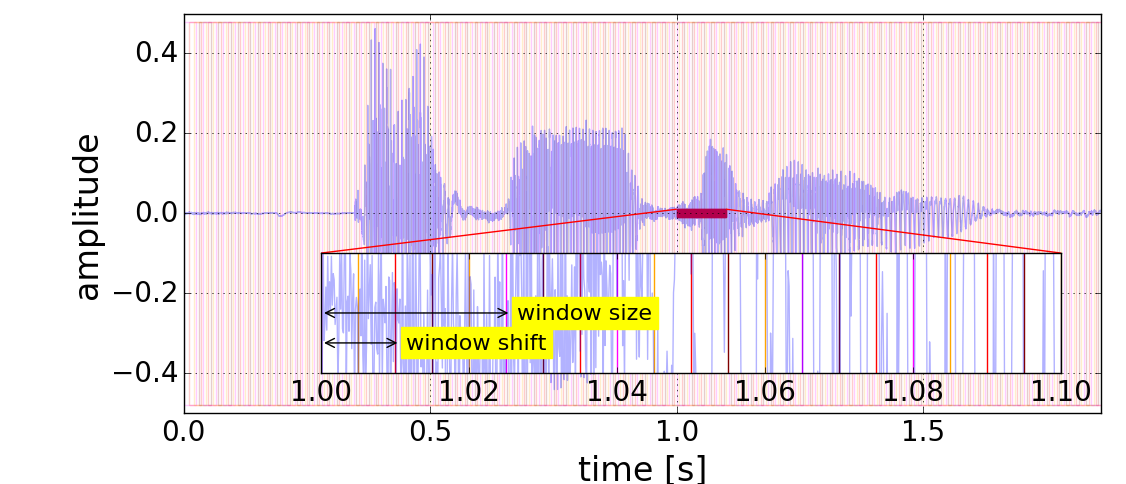
\includegraphics[width=\textwidth]{mfcc_framing.png}
\caption{Framing a sound signal.}
\label{fig:methods:mfcc_framing}
\end{figure}

We assume each frame captures one possible shape of the human vocal tract and therefore is capable of carrying one phoneme only. The next steps are applied for every single frame.

\item \textit{calculation of the periodogram estimate of the power spectrum}; 

The aim is to identify which frequencies are present. In order to do so, we apply the Hamming window and perform the discrete Fourier Transform (DFT; \cref{eq:dft}).

\begin{equation} \label{eq:dft}
S(k) = \displaystyle\sum_{n=0}^{N-1} s_n \cdot e^{-2 \pi i \frac{kn}{N}}, \qquad k = 0, ..., N-1
\end{equation}

, where $ N $ (in this case $ N = 200 $) is the signal length. Then we take the absolute value $ |S(k)| $.

\item \textit{application of the mel filterbank to the power spectra, summation of the energy in each filter, taking a logarithm of the result};

Next, we use a filterbank of triangle filters (illustrated in \cref{fig:methods:mfcc_filterbank}) predefined on the transmitted band ($ bw = \frac{f_s}{2} = 4kHz $) to get a single value per filter. We use $ 40 $ filters, therefore, each frame is now described by a vector of $ 40 $ numbers.

\begin{figure}[H]
\centering
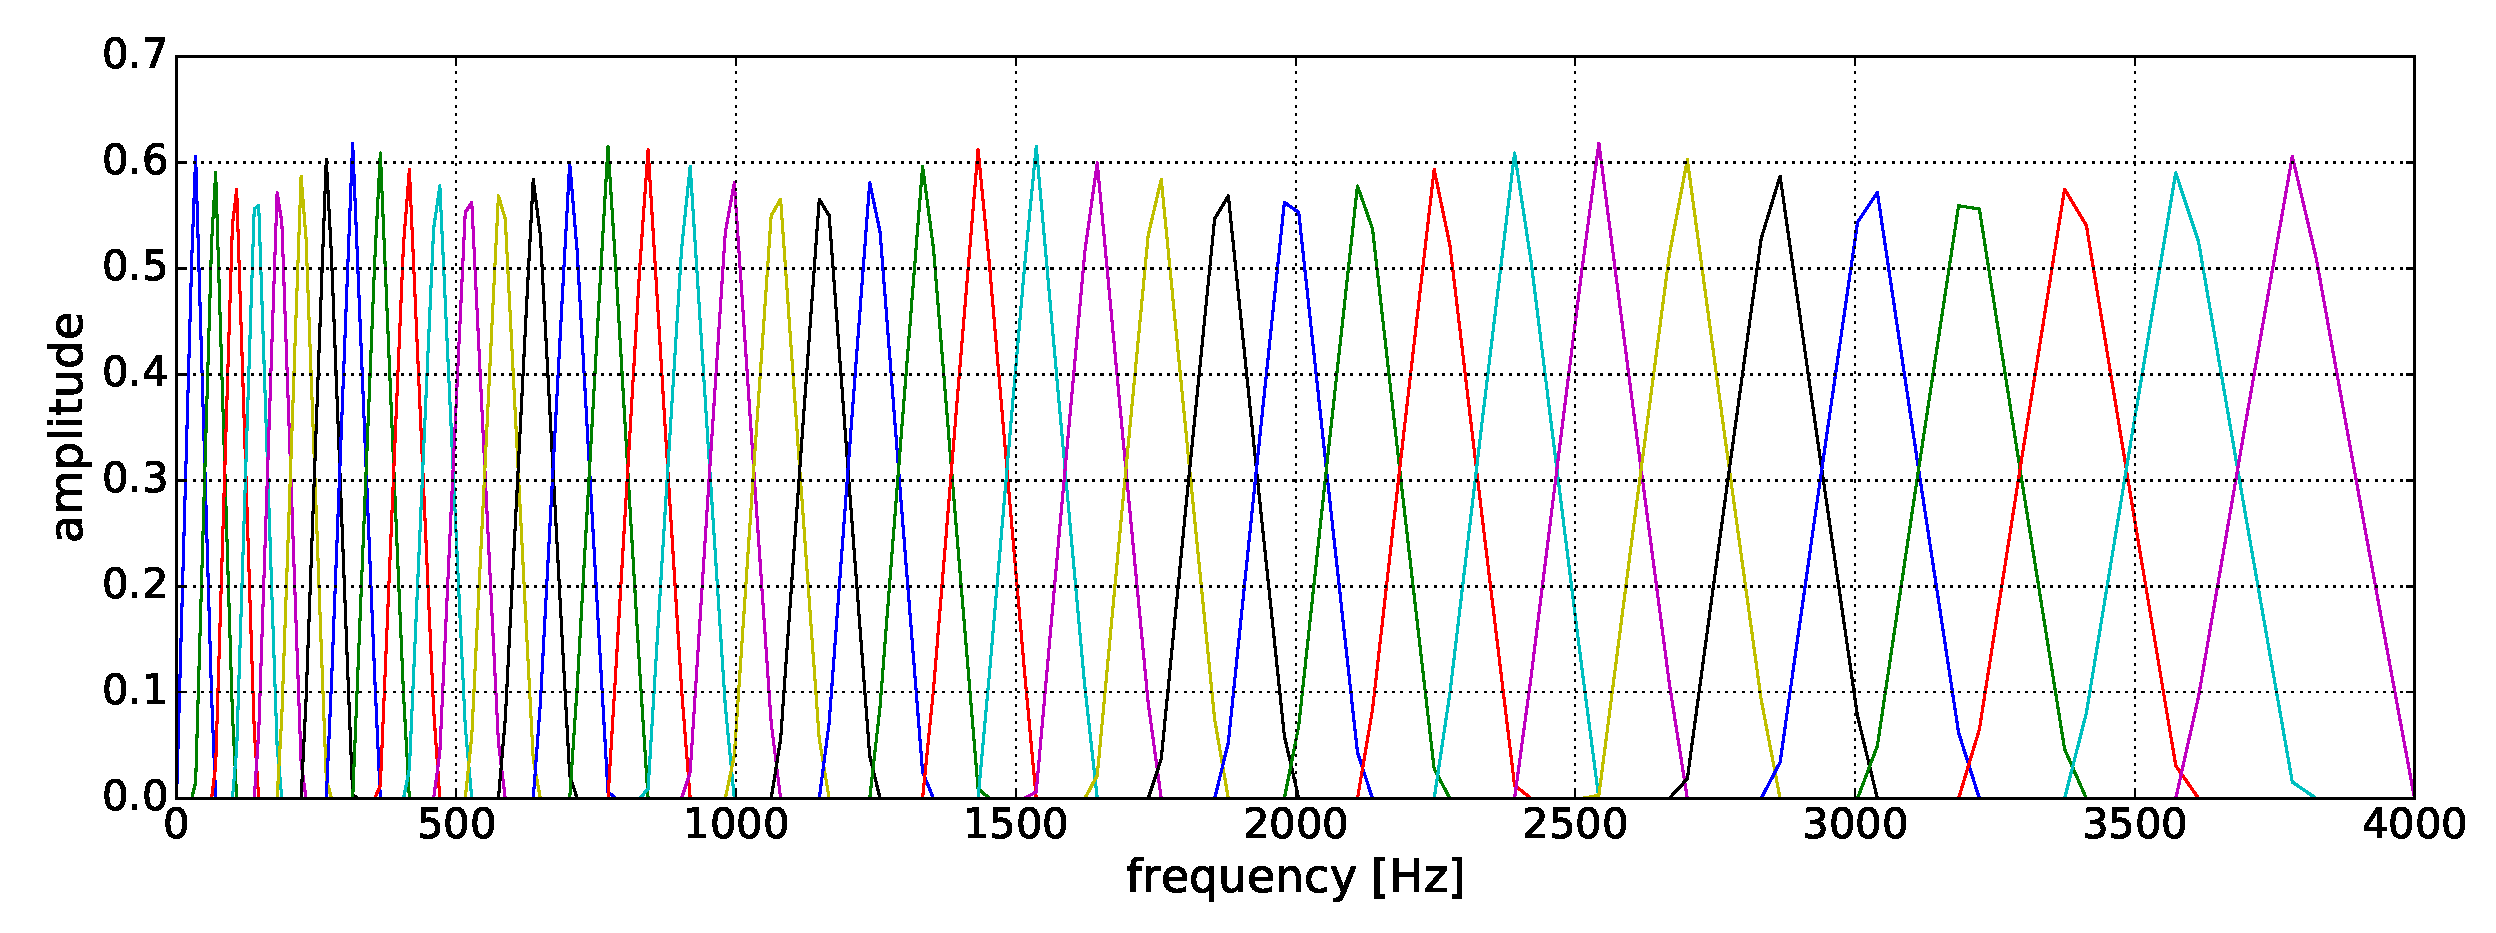
\includegraphics[width=\textwidth]{mfcc_filterbank}
\caption{Mel Filterbank of 40 filters in Hertz-axis.}
\label{fig:methods:mfcc_filterbank}
\end{figure}

Finally, a logarithm of the result is taken and considered as a description of the frame (phoneme). Usually, a discrete Cosine Transform (DCT) is applied at the end, however, it is not done in this work. The result of a signal parameterization is a matrix shown in \cref{eq:parameterization_result}.

\begin{equation} \label{eq:parameterization_result}
recording\_params = 
\begin{bmatrix}
    f_{11} & f_{12} & f_{13} & \dots  & f_{1F} \\
    f_{21} & f_{22} & f_{23} & \dots  & f_{2F} \\
    \vdots & \vdots & \vdots & \ddots & \vdots \\
    f_{W1} & f_{W2} & f_{W3} & \dots  & f_{WF}
\end{bmatrix}
\end{equation}

, where $ F = 40 $ is the number of filters and $ W $ is the number of frames (windows) depending on the duration of a recording. Value $ f_{12} $ then belongs to the feature computed with the second filter in the first frame.
\end{enumerate}

\subsection*{Data Labeling}
We perform a supervised learning method, hence the data must be labeled. To the so a speech recognition method based on Hidden Markov Models (HMMs) from \citep{smidl_pc} is used. It labels the frames of each recording as shown on an example in \cref{tab:methods:labeling_example}.

\begin{table}[H]
\centering
\begin{tabular}{|c|c|c|}
\hline
\multicolumn{3}{|c|}{recording\_name}                                                                                     \\ \hline
\multicolumn{1}{|l|}{\textit{frame\_in}} & \multicolumn{1}{l|}{\textit{frame\_out}} & \multicolumn{1}{l|}{\textit{phoneme}} \\ \hline
0                                       & 16                                      & \_sil\_                               \\ \hline
16                                      & 25                                      & a                                     \\ \hline
25                                      & 32                                      & n                                     \\ \hline
32                                      & 44                                      & o                                     \\ \hline
44                                      & 65                                      & \_sil\_                               \\ \hline
\end{tabular}
\caption{Example of labeled recording.}
\label{tab:methods:labeling_example}
\end{table}

It says that features extracted from this recording consist of $ 9 $ fourty-dimensional vectors representing phoneme \texttt{"a"}, $ 7 $ vectors of phoneme \texttt{"n"}, etc.

\subsection*{Forming a Sample}
The $ 40 $ phonemes listed in \cref{tab:methods:phonetic_alphabet} are naturally labels of classes, so we have a fourty-class classification problem. Having the information from previous section, one can match the extracted features with corresponding phonemes (classes). Now the task is to define the form of one sample.

\cref{fig:methods:sample_forming_bs} goes with the example in \cref{tab:methods:labeling_example}. The numbers in the first line are frame indices. The second line contains the known frame labels, where each frame is described by a vector of $ 40 $ features.

There is a possibility to take all frames labeled as \texttt{"a"} and consider the corresponding vectors directly as samples. However, as the labeling was not done manually and therefore cannot be considered as $ 100\% $ correct, we introduce a parameter called \texttt{border\textunderscore size}. \cref{fig:methods:sample_forming_bs} shows that we omit the frames on borders with another phoneme label and take only those in the middle.

\begin{figure}[H]
\centering
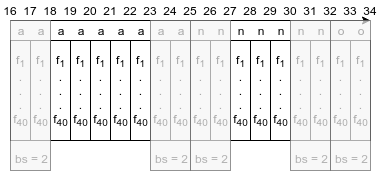
\includegraphics[width=0.8\textwidth]{sample_forming_bs}
\caption{Forming a sample, illustration of parameter \texttt{border\textunderscore size (bs)}.}
\label{fig:methods:sample_forming_bs}
\end{figure}

Moreover, in \cref{fig:methods:sample_forming_cs} parameter \texttt{context\textunderscore size} is introduced. The idea is to consider not only the information of one frame, but also of its context, into one sample.

\begin{figure}[H]
\centering
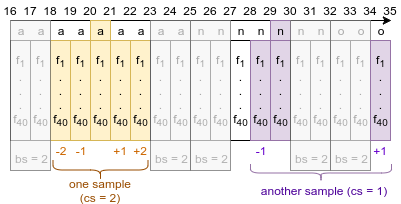
\includegraphics[width=0.75\textwidth]{sample_forming_cs}
\caption{Forming a sample, illustration of parameter \texttt{context\textunderscore size (cs)}.}
\label{fig:methods:sample_forming_cs}
\end{figure}

Based on the chosen context size $ cs $ the previous and subsequent vectors are added one by one and forms one feature vector of length $ 40 \cdot (2cs+1) $. An example for $ cs = 2 $ is illustrated in \cref{fig:methods:feature_vector}.

\begin{figure}[H]
\centering
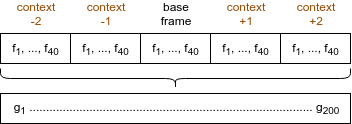
\includegraphics[width=0.8\textwidth]{feature_vector}
\caption{Example of building a feature vector with \texttt{context\textunderscore size} $ cs = 2 $.}
\label{fig:methods:feature_vector}
\end{figure}

Talking about \cref{fig:methods:feature_vector}, features $ g_1, g_2, ..., g_{200} $ gives the final feature vector of one sample, which takes the label of the base frame.

The last parameter of the speech dataset generation is the number of samples per class (\texttt{n\textunderscore samples}). The rule of thumb is the more samples the better training results, however, getting best possible training results is not the objective of this work. Therefore we often use less samples to speed up the training process.

To summarize this section, we end up with three parameters of the speech dataset generation process:

\begin{itemize}
\item \texttt{border\textunderscore size} (see \cref{fig:methods:sample_forming_bs})
\item \texttt{context\textunderscore size} (see \cref{fig:methods:sample_forming_cs})
\item \texttt{n\textunderscore samples} per class
\end{itemize}

\subsection*{Splitting data into three disjunctive sets}
\cref{fig:methods:three_sets} shows a general approach of data splitting in machine learning. It is used for all classification problems in this work. The training data is used to set up model parameters. Development data is then used for testing during the training process, in order to adjust some learning parameters based on the test results. Finally, a trained model is tested on never-seen testing data. We use splitting: $ 80\% $ training set; $ 10\% $ development set; $ 10\% $ testing set.

\begin{figure}[H]
\centering
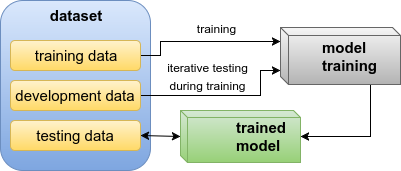
\includegraphics[width=0.7\textwidth]{three_sets}
\caption{Using three disjunctive sets of data for a general machine learning process.}
\label{fig:methods:three_sets}
\end{figure}